\documentclass[conference]{IEEEtran}

\usepackage{newtxtext,newtxmath}
\usepackage{amsmath}
\usepackage{booktabs}
\usepackage{graphicx}
\usepackage{array}
\usepackage{url}
\usepackage[hidelinks]{hyperref}

\urlstyle{tt}
\setlength{\emergencystretch}{3em}
\newcommand{\codepath}[1]{{\Urlmuskip=0mu plus 1mu\relax\nolinkurl{#1}}}
\graphicspath{{../docs/figures/ppo_pilot/}}

\begin{document}

\title{A Proximal Policy Optimization Scheduler for Joint Ramp and Peak
Reduction: Method and Three-Seed Pilot (Draft)}

\author{\IEEEauthorblockN{Janusz Gal}
\IEEEauthorblockA{jgal@charlotte.edu}}

\maketitle

\begin{IEEEkeywords}
proximal policy optimization, reinforcement learning, data centers, grid
ramp, net-load peak
\end{IEEEkeywords}

\section{Introduction}
\label{sec:introduction}

The problem-statement chapter defines a causal hourly scheduler for four
synthetic data centers. Each month, it must minimize a joint score
\(J_e\) that adds scaled one-hour ramp impact and scaled regional peak
impact, while every service arrival runs immediately, batch work finishes
within 24 hours, and no site exceeds its capacity. It compares every schedule
with the no-flexibility baseline \(\mu_{\mathrm{NF}}\), which runs all work at
its origin in its arrival hour.

This chapter describes how we solve that problem with proximal policy
optimization (PPO) and reports a first pilot: three independently trained
policies evaluated on May 2025. Section~\ref{sec:primer} introduces the
reinforcement-learning terms as they apply to this problem.
Section~\ref{sec:ppo} explains PPO. Section~\ref{sec:running} describes how a
training run works and what a seed controls. Sections~\ref{sec:evaluation}
and~\ref{sec:results} give the evaluation protocol and results. The pilot is a
draft result: it has three seeds and one validation month.

\section{Reinforcement Learning for This Problem}
\label{sec:primer}

\subsection{Agent, environment, and episodes}

Reinforcement learning trains an \emph{agent} to choose actions that
maximize the total \emph{reward} it collects from an
\emph{environment} \cite{sutton2018reinforcement}. Here the agent is the
scheduler and the environment is the simulated four-site fleet with its grid
data.\footnote{The environment is \codepath{RampAwareEnv} in
\codepath{env/ramp_v6/environment.py}. \codepath{make_four_market_env} in
\codepath{energy_model_v3/four_market_v2.py} builds it from the generated
factory.} One interaction is one decision hour: the agent observes the state
of the grid and its queues, chooses an action, and receives a reward once the
hour's realized net load is known.

An \emph{episode} is one calendar month of 672 to 744 hours. Queues and
site-power history carry across midnight, and the episode ends at month-end
with every queue empty. Training cycles through the eleven training months;
May is never seen during training.

\subsection{Observation}

The agent sees an 82-number \emph{observation}, the information set
\(\mathcal I_t\) from the problem statement.\footnote{\codepath{_build_observation_schema}
and \codepath{_observation} in \codepath{env/ramp_v6/environment.py} define
and fill the 82 entries.} For each of the four markets, it contains
standardized gross demand and net load for hour \(t-1\); the four gross-demand
and four net-load forecasts issued at \(t-1\); the steepest forecast climb for
each quantity; and the running adjusted and original peaks. For each site, it
contains the hour-\(t\) service and batch arrivals, the queued batch work, and
the previous hour's power. It ends with five queue-urgency totals, the hour of
day and day of week as sine--cosine pairs, and the fraction of the month
remaining. No entry comes from hour \(t\) or later.

\subsection{Action}

The action is nine bounded numbers in \([-6,6]\): four service preferences,
one batch-release level, and four batch-destination
preferences.\footnote{\codepath{action_schema} in
\codepath{env/ramp_v6/environment.py} names the nine entries, and
\codepath{project_action} in \codepath{env/ramp_v6/projection.py} decodes
them.} A decoder turns them into a feasible schedule every hour:
\begin{itemize}
  \item a softmax of the service preferences splits total service among the
        sites, then a projection keeps each site within capacity;
  \item the release level maps linearly from \([-6,6]\) to a fraction
        \([0,1]\) of the batch queue, raised when needed to meet deadlines
        and capped by spare capacity; and
  \item a softmax of the destination preferences places that batch work, and
        earliest-deadline-first order decides whose work it is.
\end{itemize}
The decoder guarantees the service, deadline, and capacity constraints, so the
agent never needs a penalty to learn them. It can only express preferences
among feasible schedules.

\subsection{Reward and return}

Each hour's reward is that hour's share of \(-J_e\):
\begin{equation}
  r_t
  =
  -\frac{0.5}{C_R}\sum_{m} I_{m,t}
  -\frac{0.5}{C_Q}\sum_{m}\left[
    \left(M_{m,t}-M_{m,t-1}\right)
    -\left(O_{m,t}-O_{m,t-1}\right)
  \right],
  \label{eq:reward}
\end{equation}
where \(I_{m,t}\) is the ramp impact and \(M_{m,t}\) and \(O_{m,t}\) are the
running normalized adjusted and original peaks, starting from zero. Running
maxima telescope, so the month's undiscounted \emph{return} is exactly
\(\sum_t r_t=-J_e\).\footnote{\codepath{JointObjective.reward_components} in
\codepath{env/ramp_v6/objective.py} computes both terms, and
\codepath{tests/ramp_v6/test_joint_objective.py} checks that a month of
rewards equals \(-J_e\).} Maximizing return is therefore the same as
minimizing \(J_e\).

\subsection{Policy and value function}

A \emph{policy} \(\pi_\theta(a\mid o)\) maps an observation to a probability
distribution over actions. Ours is a neural network with parameters
\(\theta\). A \emph{value function} \(V_\phi(o)\) estimates the discounted
return expected from an observation; it is used only during training, to judge
whether an action did better or worse than expected. PPO trains both
together, an arrangement called actor--critic.

\section{Proximal Policy Optimization}
\label{sec:ppo}

\subsection{Why PPO}

PPO \cite{schulman2017ppo} is a policy-gradient method: it adjusts \(\theta\)
in the direction that makes better-than-expected actions more likely. It
handles continuous actions directly, needs no model of grid dynamics, and
usually works with standard settings. We use the Stable-Baselines3
implementation \cite{raffin2021sb3}.\footnote{Version 2.9.0, pinned in
\codepath{requirements.txt}; \codepath{ramp_rl/runner.py} refuses to run with
any other version.}

\subsection{Collecting experience}

Training alternates two phases. In the \emph{rollout} phase, the current
policy runs in the simulator and records observations, actions, rewards, and
value estimates. Actions are sampled from a diagonal Gaussian distribution
whose mean the network outputs and whose per-dimension standard deviation is
learned separately. That randomness is how the agent explores. Samples are
clipped to \([-6,6]\) before the decoder sees them.

\subsection{Advantages}

After a rollout, generalized advantage estimation \cite{schulman2016gae}
measures how much better each action turned out than the value function
predicted:
\begin{align}
  \delta_t &= r_t+\gamma V_\phi(o_{t+1})-V_\phi(o_t),
  \label{eq:td-error}\\
  \hat A_t &= \sum_{l\geq0}(\gamma\lambda)^l\,\delta_{t+l},
  \label{eq:gae}
\end{align}
with discount \(\gamma=0.99\) and \(\lambda=0.95\). The sum stops at the end of
an episode. Advantages are normalized within each minibatch.

The discount means a reward 100 hours away counts about 37\% as much as one
now. \(J_e\) itself is undiscounted, so PPO optimizes a close approximation of
the objective rather than the objective exactly. The approximation matters
most for peaks set late in a month by decisions made much earlier.

\subsection{The clipped update}

In the \emph{update} phase, PPO improves the policy using the recorded
experience. With the probability ratio
\(\rho_t(\theta)=\pi_\theta(a_t\mid o_t)/\pi_{\theta_{\mathrm{old}}}(a_t\mid o_t)\),
it maximizes
\begin{equation}
  L^{\mathrm{clip}}(\theta)
  =
  \mathbb{E}_t\!\left[
    \min\!\left(
      \rho_t\hat A_t,\;
      \mathrm{clip}(\rho_t,1-\epsilon,1+\epsilon)\,\hat A_t
    \right)
  \right],
  \label{eq:ppo-clip}
\end{equation}
with \(\epsilon=0.2\). The clip removes any gain from moving an action's
probability more than 20\% away from the policy that collected the data, so
each update stays close to experience the agent actually has. The value
network is trained to match observed returns with squared error, weighted
0.5 in the combined loss. There is no entropy bonus, and gradients are
clipped to norm 0.5.

\subsection{Normalization}

Observations and rewards have very different scales, so training wraps the
environments in a running normalizer.\footnote{\codepath{VecNormalize} from
Stable-Baselines3, created in \codepath{run_training} in
\codepath{ramp_rl/runner.py} and saved beside each model as
\codepath{vecnormalize.pkl}.} Each observation entry is standardized with a
running mean and variance and clipped to \(\pm10\). Rewards are divided by a
running standard deviation of the discounted return and clipped to \(\pm10\).
Normalization only rescales what the network sees. The recorded rewards and
every reported \(J_e\) use raw, unnormalized values.

\subsection{Network and hyperparameters}

Table~\ref{tab:hyperparameters} lists the settings. The policy and value
networks are separate, each with two hidden layers of 64 tanh units, for
19,603 trainable parameters in total. We have not tuned these settings.

\begin{table}[htbp]
  \centering
  \footnotesize
  \caption{PPO settings used in the pilot.}
  \label{tab:hyperparameters}
  \begin{tabular}{@{}lr@{}}
    \toprule
    Setting & Value \\
    \midrule
    Parallel environments & 4 \\
    Steps per environment per rollout & 512 \\
    Transitions per update & 2,048 \\
    Epochs per update & 10 \\
    Minibatch size & 256 \\
    Learning rate (Adam) & \(3\times10^{-4}\) \\
    Discount \(\gamma\) & 0.99 \\
    GAE \(\lambda\) & 0.95 \\
    Clip range \(\epsilon\) & 0.2 \\
    Value-loss weight & 0.5 \\
    Entropy bonus & 0 \\
    Gradient-norm limit & 0.5 \\
    Hidden layers (policy, value) & 64, 64 (tanh) \\
    Initial action standard deviation & 1 \\
    Interactions per run & 1,024,000 \\
    \bottomrule
  \end{tabular}
\end{table}

\section{Running a Training Run}
\label{sec:running}

\subsection{What one run does}

A run trains one policy from scratch.\footnote{\codepath{run_training} in
\codepath{ramp_rl/runner.py}. Its PPO settings come from the
\codepath{training} section of \codepath{env/protocols/four_market_v2.yaml}.}
Four copies of the environment step in turn inside one process. Each rollout
collects 512 hours from each copy, 2,048 transitions in all. PPO then makes 10
passes over those transitions in minibatches of 256, 80 gradient steps per
update.

A request for 1,000,000 interactions is rounded up to the next checkpoint
boundary, 1,024,000 interactions or 500 updates. Each copy sees 256,000 hours,
about 351 simulated months, so a run covers roughly 1,400 months, or about 128
passes through the training year. Each copy draws the eleven training months
in a freshly shuffled order before repeating any of them.\footnote{\codepath{FourMarketV2WindowEnv._next_window_id}
in \codepath{energy_model_v3/four_market_v2.py}.}

\subsection{Checkpoints and logs}

After every rollout, the run appends one row of raw training metrics to a
learning-curve file. Every 25 rollouts (51,200 interactions), it saves a
resumable checkpoint. It also keeps milestone snapshots at the first
checkpoints past 110,592, 500,000, and 1,000,000
interactions.\footnote{\codepath{TrainingCallback} and
\codepath{save_latest_checkpoint} in \codepath{ramp_rl/runner.py}. A
checkpoint records the environment identity, PPO settings, and seed, and a
resumed run must match all three.} Each checkpoint stores the objective
version, data digest, and observation and action shapes, so a model can never
be evaluated against a different objective or data set.\footnote{\codepath{environment_identity}
in \codepath{ramp_rl/contract.py}; \codepath{tests/ramp_v6/test_campaign_instrumentation.py}
tests checkpointing and resumption.}

\subsection{What a seed is}

A seed is the integer that fixes every random choice in one run. Seed \(s\)
sets the Python, NumPy, and PyTorch generators and the PPO seed, which
determine the network's initial weights, the exploration noise, and the
minibatch shuffling. Environment copy \(r\) receives seed \(s+r\) and shuffles
its month order with a generator seeded by \(s+1009r\).\footnote{\codepath{_make_vec_env}
and \codepath{run_training} in \codepath{ramp_rl/runner.py}.}

Everything else is identical across seeds: the data, objective, constraints,
and hyperparameters. Differences between seeds therefore measure how much the
result depends on the randomness of training, not uncertainty about future
grids or workloads. A single seed can be lucky or unlucky; several seeds show
whether a result is repeatable. The pilot uses seeds 4101--4103. The planned
campaign uses ten, 4101--4110.

\subsection{Commands}

From the repository root, the pilot is reproduced with three
commands:\footnote{\codepath{scripts/build_four_market_v2_factory.py} builds
the monthly fixtures, \codepath{scripts/run_four_market_v2_pilot.py} trains and
evaluates the seeds, and \codepath{scripts/build_ppo_pilot_figures.py} draws the
figures in this chapter.}
{\footnotesize
\begin{verbatim}
python scripts/build_four_market_v2_factory.py
python scripts/run_four_market_v2_pilot.py \
    --seeds 4101 4102 4103 \
    --timesteps 1000000 --tag impact-50-50-1m
python scripts/build_ppo_pilot_figures.py \
    --tag impact-50-50-1m
\end{verbatim}
}
The pilot script trains the seeds in parallel processes and evaluates every
milestone. It writes learning curves and summaries to
\codepath{output/four_market_joint_v3/pilot/impact-50-50-1m/} and checkpoints
to \codepath{models/four_market_joint_v3/pilot/impact-50-50-1m/}. The option
\codepath{--ramp-weight} selects ramp-only (1) or peak-only (0) variants of the
objective. The full ten-seed campaign uses
\codepath{scripts/run_four_market_v2_campaign.py}.

On an eight-core laptop, each seed trained at about 240 interactions per
second and finished in 71--72 minutes, with the three seeds running at once.

\section{Evaluation Protocol}
\label{sec:evaluation}

Each saved policy is evaluated on May 2025, one continuous 744-hour
episode.\footnote{\codepath{evaluate_checkpoint} and \codepath{_run_episode}
in \codepath{ramp_rl/evaluation.py}.} Evaluation differs from training in
three ways. The policy acts \emph{deterministically}, using the mean of its
Gaussian rather than sampling. The normalizer's statistics are frozen at their
training values. And the no-flexibility baseline runs on the same 744 hours,
with the same arrivals, grid data, and forecasts.

We report \(J_e(\mu_{\mathrm{NF}})-J_e(\mu)\), positive when PPO improves on
the baseline, together with its ramp and peak parts. For the final
checkpoints we also recomputed \(J_e\) independently from the raw panel and
each site's power; it matched the environment's return exactly, with no
service, deadline, or capacity violation.

May also informed the choice of forecast lead times, so it is a validation
month rather than an untouched test set.

\section{Pilot Results}
\label{sec:results}

\subsection{Training}

Fig.~\ref{fig:learning} shows the return of each completed training month.
All three seeds begin below the baseline, because random exploration moves
power erratically, and cross the baseline's level within about 50,000
interactions. Returns rise quickly to about 0.010 by 400,000 interactions and
then climb slowly to 0.013--0.014. The three curves are nearly
indistinguishable.\footnote{Learning-curve data:
\codepath{learning_curve.csv} in each seed's output folder. Figures are drawn by
\codepath{scripts/build_ppo_pilot_figures.py}, which writes every quoted number
to \codepath{docs/figures/ppo_pilot/figure_data.json}.}

\begin{figure}[!t]
  \centering
  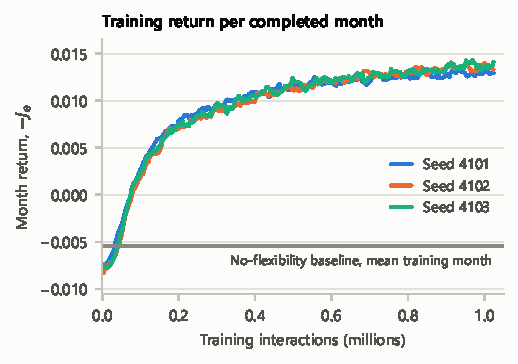
\includegraphics[width=\columnwidth]{learning_curves.pdf}
  \caption{Return of each completed training month (\(-J_e\), higher is
  better), as a 10-rollout rolling mean. The gray line is the no-flexibility
  baseline's return averaged over the eleven training months,
  \(-0.00544\).}
  \label{fig:learning}
\end{figure}

\subsection{May improvement}

Table~\ref{tab:may} and Fig.~\ref{fig:checkpoints} give the May results. The
baseline scores \(J_e=0.005613\). Every checkpoint of every seed improves on
it, and the final policies reach \(J_e\) between \(-0.0097\) and
\(-0.0114\), improvements of 0.0153 to 0.0170. Both terms of
\(J_e\) are measured against the original grid without the fleet, which is
why \(J_e\) can be negative. The ramp term falls below zero when the fleet
smooths ramps. The peak term cannot: any site power lifts a region's monthly
peak above the original grid's, so \(\Phi_{m,e}>0\). Because the original peak
is fixed, minimizing \(\Phi_{m,e}\) is the same as minimizing each region's
highest adjusted net load, and the policies lower that added peak by about a
quarter relative to the baseline.

\begin{table}[htbp]
  \centering
  \footnotesize
  \caption{May improvement \(J_e(\mu_{\mathrm{NF}})-J_e(\mu)\) by checkpoint,
  and the split of the final improvement into its weighted ramp and peak
  parts.}
  \label{tab:may}
  \begin{tabular}{@{}lrrr@{}}
    \toprule
    & Seed 4101 & Seed 4102 & Seed 4103 \\
    \midrule
    153,600 interactions   & 0.0131 & 0.0125 & 0.0134 \\
    512,000 interactions   & 0.0155 & 0.0155 & 0.0162 \\
    1,024,000 interactions & 0.0153 & 0.0165 & 0.0170 \\
    \midrule
    Final \(J_e(\mu)\)     & \(-0.0097\) & \(-0.0109\) & \(-0.0114\) \\
    Ramp part              & 0.0139 & 0.0152 & 0.0155 \\
    Peak part              & 0.0014 & 0.0013 & 0.0016 \\
    \bottomrule
  \end{tabular}
\end{table}

\begin{figure}[!t]
  \centering
  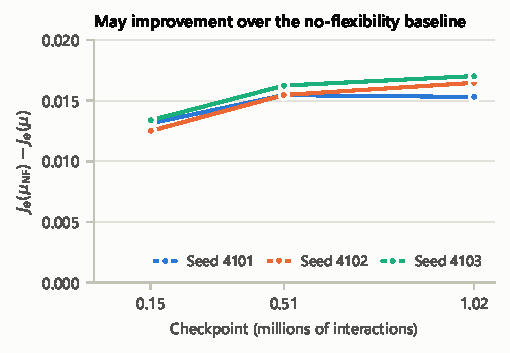
\includegraphics[width=\columnwidth]{checkpoint_improvement.pdf}
  \caption{May improvement over the no-flexibility baseline at each saved
  checkpoint.}
  \label{fig:checkpoints}
\end{figure}

About 90\% of the improvement comes from ramps. The fleet's total squared
one-hour ramp, relative to the original grid, falls by 2.8--3.1\%. The peak
impact \(\sum_m\Phi_{m,e}\) falls from 0.0411 under the baseline to
0.0296--0.0316, a cut of about a quarter. The ramp gain is mostly in place by
153,600 interactions, while the peak gain roughly doubles between the first
and last checkpoints.

\subsection{Regions}

Fig.~\ref{fig:regions} and Table~\ref{tab:regions} break the result down by
region. ISO-NE NEMA, where a site's power range is largest relative to typical
ramps, gains most: its squared ramp falls 11--14\% and its monthly peak falls
109--140 MW. CAISO NP15 and SPP North improve on both measures. MISO
Minnesota, where a site's power is smallest relative to the grid, changes
little, and its peak rises by up to 35 MW in two seeds.

\begin{figure*}[!t]
  \centering
  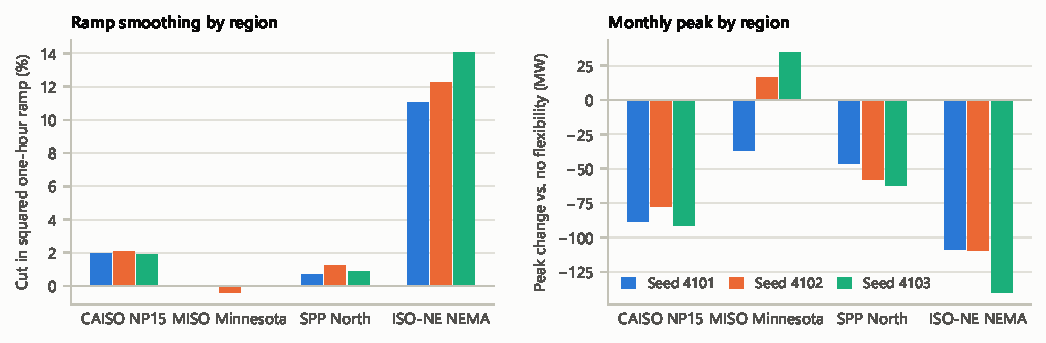
\includegraphics[width=\textwidth]{regional_results.pdf}
  \caption{May results by region for the final policies. Left: percentage
  cut in the total squared one-hour ramp relative to the original grid. Right:
  change in the monthly adjusted net-load peak relative to the no-flexibility
  baseline; negative is a reduction.}
  \label{fig:regions}
\end{figure*}

\begin{table*}[htbp]
  \centering
  \footnotesize
  \caption{Regional May results for the final policies.}
  \label{tab:regions}
  \begin{tabular}{@{}lrrrrrr@{}}
    \toprule
    & \multicolumn{3}{c}{Squared-ramp cut (\%)}
    & \multicolumn{3}{c}{Peak change vs.\ baseline (MW)} \\
    \cmidrule(lr){2-4}\cmidrule(l){5-7}
    Market case & 4101 & 4102 & 4103 & 4101 & 4102 & 4103 \\
    \midrule
    CAISO NP15     & 2.0  & 2.1  & 1.9  & \(-88\)  & \(-78\)  & \(-91\) \\
    MISO Minnesota & 0.0  & \(-0.4\) & 0.0 & \(-37\) & \(+16\) & \(+35\) \\
    SPP North      & 0.7  & 1.2  & 0.9  & \(-46\)  & \(-58\)  & \(-62\) \\
    ISO-NE NEMA    & 11.0 & 12.2 & 14.1 & \(-109\) & \(-109\) & \(-140\) \\
    \bottomrule
  \end{tabular}
\end{table*}

\subsection{How the policies act}

The policies work mainly by moving service between sites. About 31\% of May's
service work runs away from its origin site, while batch work waits only
1.0--1.5 hours on average despite its 24-hour window. The decoder changes the
requested allocation in 68--75\% of hours. It does so when a request exceeds
spare capacity or the queue, or releases less batch work than deadlines
require.

Fig.~\ref{fig:isone} shows ISO-NE over three days around its May peak hour.
Under the baseline, site power stays near 340 MW. The PPO policy instead runs
the site near full power while net load is low and cuts it to about 200 MW as
net load climbs to its evening peak. At the peak hour it draws 231 MW, 109 MW
less than the baseline.

\begin{figure*}[!t]
  \centering
  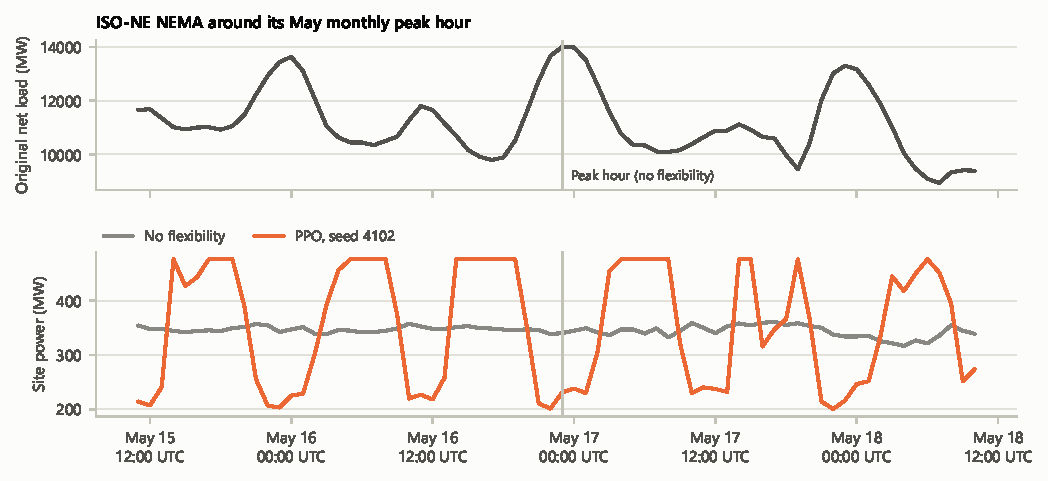
\includegraphics[width=\textwidth]{isone_peak_window.pdf}
  \caption{ISO-NE NEMA from 15 to 18 May 2025. Top: original net load. Bottom:
  site power under the no-flexibility baseline and the seed-4102 policy. The
  vertical line marks the baseline's monthly peak hour, 16 May 23:00 UTC.}
  \label{fig:isone}
\end{figure*}

\section{Limitations and Next Steps}
\label{sec:limitations}

\begin{itemize}
  \item \emph{Few seeds, one month.} Three seeds and a single validation month
        show that the result repeats, but cannot yet support statistical
        claims. The planned campaign uses ten seeds.
  \item \emph{No objective ablation.} We have not yet trained ramp-only or
        peak-only policies. Without them we cannot say how much of the peak
        reduction the peak term itself causes; a ramp-only policy may reduce
        peaks too.
  \item \emph{Nominal weights.} The 0.5 weights are applied to scaled terms,
        but the fleet can move the ramp term far more than the peak term, so
        the objective weights ramps more heavily in practice.
  \item \emph{Discounting.} PPO maximizes a discounted return with
        \(\gamma=0.99\), an approximation of the undiscounted \(J_e\).
  \item \emph{Untuned training.} The hyperparameters are common defaults, not
        tuned for this problem.
  \item \emph{Optimistic routing.} Moving work between sites is free and
        instant, so the results are an upper bound on geographic
        flexibility.
  \item \emph{No simple heuristic.} We compare only with the no-flexibility
        baseline, not with a rule-based scheduler that uses the same
        forecasts.
\end{itemize}

\begin{thebibliography}{99}

\bibitem{sutton2018reinforcement}
R. S. Sutton and A. G. Barto, \emph{Reinforcement Learning: An Introduction},
2nd ed. Cambridge, MA, USA: MIT Press, 2018.

\bibitem{schulman2017ppo}
J. Schulman, F. Wolfe, P. Dhariwal, A. Radford, and O. Klimov, ``Proximal
policy optimization algorithms,'' arXiv:1707.06347, 2017.

\bibitem{schulman2016gae}
J. Schulman, P. Moritz, S. Levine, M. Jordan, and P. Abbeel,
``High-dimensional continuous control using generalized advantage
estimation,'' in \emph{Proc. Int. Conf. Learn. Represent. (ICLR)}, 2016.

\bibitem{raffin2021sb3}
A. Raffin, A. Hill, A. Gernhardt, M. Ernestus, and N. Dormann,
``Stable-Baselines3: Reliable reinforcement learning implementations,''
\emph{J. Mach. Learn. Res.}, vol. 22, no. 268, pp. 1--8, 2021.

\end{thebibliography}

\end{document}
